Шейдер (англ. shader — затеняющая программа) -- компьютерная программа, предназначенная для исполнения процессорами видеокарты (GPU).
Шейдеры составляются на одном из специализированных языков программирования и компилируются в инструкции для GPU. Шейдеры необходимы, когда требуется что-то нарисовать
с помощью WebGL. 
Сначала видеокарты оснащали несколькими специализированными процессорами, поддерживающими разные наборы инструкций. Шейдеры делили на три типа в зависимости от того,
какой процессор будет их исполнять (в зависимости от того, какие наборы инструкций доступны):
\begin{itemize}
\item вершинный шейдер (vertex shader): вершинный шейдер -- это программа,описывающая характеристики вершины (координаты, цвет и другие), а вершина – это точка в двух- или 
трехмерном пространстве, например, угол или вершина двух- или трехмерной фигуры. Он оперирует данными, связанными с вершинами многогранников, например, с координатами вершины 
(точки) в пространстве, с текстурными координатами, с цветом вершины, с вектором касательной, с вектором бинормали, с вектором нормали. Вершинный шейдер может использоваться 
для видового и перспективного преобразования вершин, для генерации текстурных координат, для расчёта освещения и т. д.;
\item фрагментный шейдер (fragment shader): фрагментный шейдер -- это программа, реализующая обработку фрагментов изображений, например, определение освещенности, где под
фрагментом подразумевается простейший элемент изображения, своего рода «пиксель». Пиксельный шейдер используется на последней стадии графического конвейера для формирования фрагмента изображения.
\item геометрический шейдер (geometry shader): геометрический шейдер -- это программа. которая, в отличие от вершинного, способна обработать не только одну вершину, но и целый примитив. 
Примитивом может быть отрезок (две вершины) и треугольник (три вершины), а при наличии информации о смежных вершинах (англ. adjacency) для треугольного примитива может быть обработано до шести вершин. Геометрический шейдер 
способен генерировать примитивы «на лету» (не задействуя при этом центральный процессор).
\end{itemize}

Шейдеры обеспечивают большую гибкость и высокую реалистичность современной трехмерной графики, позволяя использовать новые эффекты отображения для достижения ошеломляющих
результатов. В данном проекте извлекаются из кода на JavaScript и сохраняются в системе WebGL, готовыми к использованию. На рисунке \ref{figure:domain:shaders} показана типовая последовательность
операций – от запуска программы JavaScript до передачи шейдеров систему WebGL, – которая применяется при рисовании фигур.

\begin{figure}[ht]
\centering
  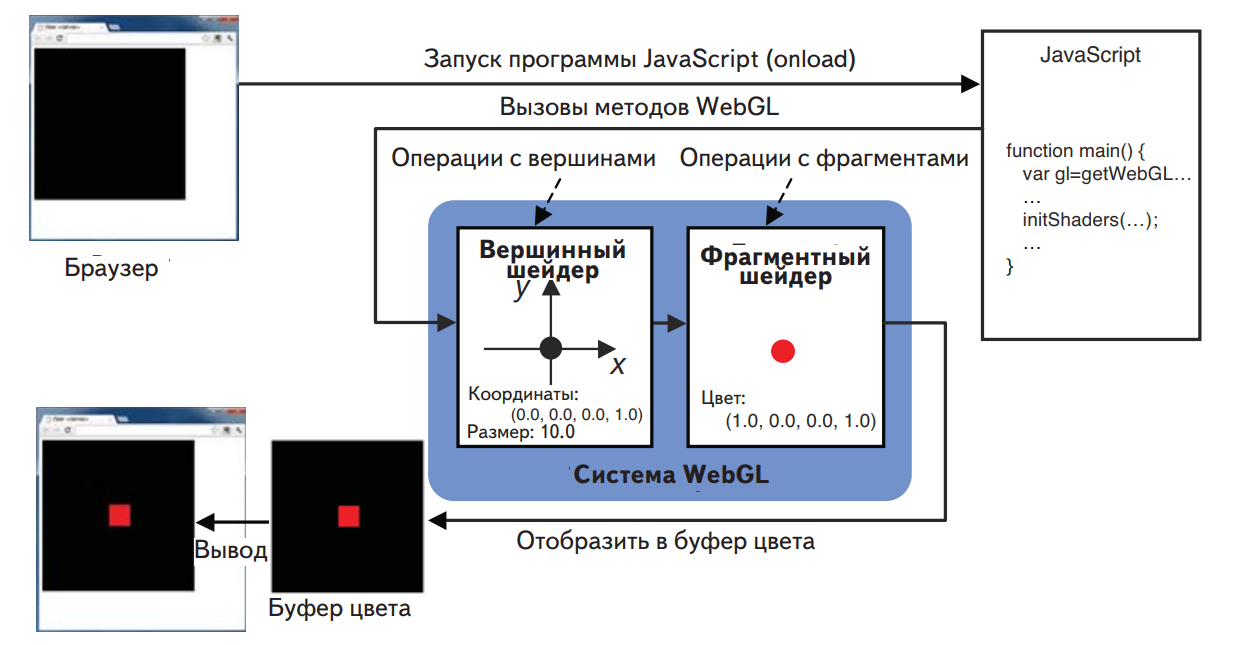
\includegraphics[scale=0.4]{shaders.png}
  \caption{Последовательность операций, от запуска программы JavaScript до отображения результатов в окне браузера}
  \label{figure:domain:shaders}
\end{figure}

Слева на рисунке  изображены два окна браузера. Это одно и то же окно в разные моменты времени. Вверху показано окно браузера перед выполнением программы JavaScript,
а внизу – то же окно, но после выполнения программы. В момент вызова методов WebGL из программы на JavaScript, система WebGL выполнит вершинный и фрагментный шейдеры, 
чтобы вывести результат в буфер цвета. Это – этап очистки. После этого содержимое буфера цвета автоматически выводится в область рисования, определяемую элементом <canvas>.

Шейдеры являются основным механизмом в системе WebGL, используемым при создании приложений трехмерной графики, а язык GLSL ES –
это самостоятельный язык программирования шейдеров для таких приложений. 

\begin{figure}[ht]
\centering
  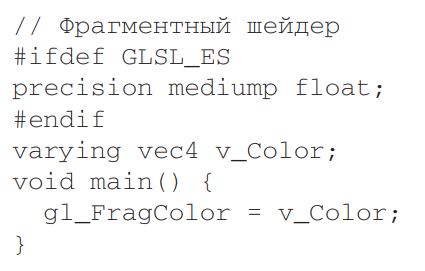
\includegraphics[scale=0.9]{pixel_shader.png}
  \caption{Пример простого фрагментного шейдера}
  \label{figure:domain:pixel_shader}
\end{figure}

